%%%%%%%%%%%%%%%%%%%%%%%%%%%%%%%%%%%%%%%%%
% Beamer Presentation
% LaTeX Template
% Version 1.0 (10/11/12)
%
% This template has been downloaded from:
% http://www.LaTeXTemplates.com
%
% License:
% CC BY-NC-SA 3.0 (http://creativecommons.org/licenses/by-nc-sa/3.0/)
%
%%%%%%%%%%%%%%%%%%%%%%%%%%%%%%%%%%%%%%%%%

%----------------------------------------------------------------------------------------
%	PACKAGES AND THEMES
%----------------------------------------------------------------------------------------

\documentclass{beamer}

\mode<presentation> {

% The Beamer class comes with a number of default slide themes
% which change the colors and layouts of slides. Below this is a list
% of all the themes, uncomment each in turn to see what they look like.

%\usetheme{default}
% \usetheme{AnnArbor}
% \usetheme{Antibes} +
% \usetheme{Bergen}
% \usetheme{Berkeley}
% \usetheme{Berlin}
% \usetheme{Boadilla}
\usetheme{CambridgeUS}
% \usetheme{Copenhagen} +
% \usetheme{Darmstadt}
% \usetheme{Dresden}
% \usetheme{Frankfurt}
% \usetheme{Goettingen}
% \usetheme{Hannover}
% \usetheme{Ilmenau}
% \usetheme{JuanLesPins}
% \usetheme{Luebeck} +
% \usetheme{Madrid}
% \usetheme{Malmoe}
% \usetheme{Marburg}
% \usetheme{Montpellier} +
% \usetheme{PaloAlto}
% \usetheme{Pittsburgh}
% \usetheme{Rochester}
% \usetheme{Singapore}
% \usetheme{Szeged}
% \usetheme{Warsaw} +

% As well as themes, the Beamer class has a number of color themes
% for any slide theme. Uncomment each of these in turn to see how it
% changes the colors of your current slide theme.

% \usecolortheme{albatross}
\usecolortheme{beaver}
% \usecolortheme{beetle}
% \usecolortheme{crane}
% \usecolortheme{dolphin}
% \usecolortheme{dove}
% \usecolortheme{fly}
% \usecolortheme{lily}
% \usecolortheme{orchid}
% \usecolortheme{rose}
% \usecolortheme{seagull}
% \usecolortheme{sidebartab}
% \usecolortheme{seahorse}
% \usecolortheme{whale}
% \usecolortheme{wolverine}

%\setbeamertemplate{footline} % To remove the footer line in all slides uncomment this line
%\setbeamertemplate{footline}[page number] % To replace the footer line in all slides with a simple slide count uncomment this line

%\setbeamertemplate{navigation symbols}{} % To remove the navigation symbols from the bottom of all slides uncomment this line
}

\usepackage{graphicx} % Allows including images
\usepackage{booktabs} % Allows the use of \toprule, \midrule and \bottomrule in tables
\usepackage[brazil]{babel}
\selectlanguage{brazil}
\languagepath{brazil}
\deftranslation[to=brazil]{Example}{Exemplo}
\deftranslation[to=brazil]{Theorem}{Teorema}
\usepackage[utf8]{inputenc}
\usepackage{amssymb}
\usepackage{mathtools}
\usepackage{pythonhighlight}

%----------------------------------------------------------------------------------------
%	TITLE PAGE
%----------------------------------------------------------------------------------------

\title[Identificação de Locutor]{Identificação de Locutor} % The short title appears at the bottom of every slide, the full title is only on the title page

\author{Ramon Duarte de Melo \& André Ribeiro Queiroz} % Your name
\institute[UFRJ] % Your institution as it will appear on the bottom of every slide, may be shorthand to save space
{
    Universidade Federal do Rio de Janeiro \\ % Your institution for the title page
    \medskip
    \textit{ramonduarte@poli.ufrj.br \& handre\_queiroz@poli.ufrj.br} \\ % Your email address
    \bigskip
    Código e apresentação disponíveis em: \texttt{https://github.com/ramonduarte/procvoz}
    
    }
    \date{\today} % Date, can be changed to a custom date

\begin{document}

\begin{frame} % SLIDE 1
    \titlepage % Print the title page as the first slide
\end{frame}

\begin{frame} % SLIDE 2
    \frametitle{Sumário} % Table of contents slide, comment this block out to remove it
    \tableofcontents 
\end{frame}

%----------------------------------------------------------------------------------------
%	PRESENTATION SLIDES
%----------------------------------------------------------------------------------------

%------------------------------------------------
% \section{O Problema} 
%------------------------------------------------

\section{Arquitetura}


\begin{frame} % SLIDE 3
    \frametitle{Visão Geral do Sistema}

    \begin{figure}
        \centering
        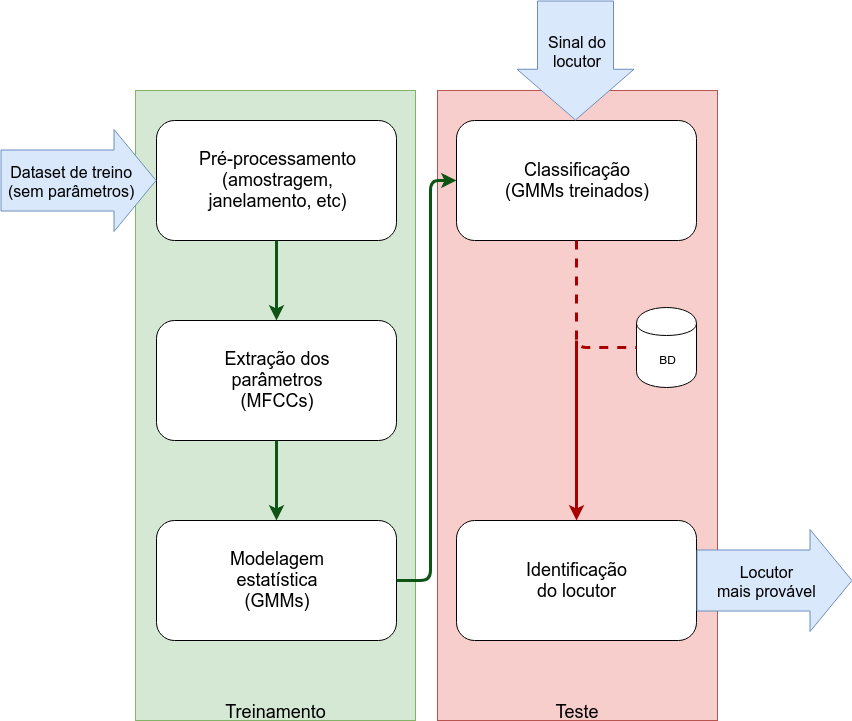
\includegraphics[height=192pt]{fig2.png}
        % \caption{Pipeline do processo de reconhecimento de locutor.}
    \end{figure}


\end{frame}


\section{Dados de entrada}

\begin{frame} % SLIDE 3
    \frametitle{Sinais de entrada (treino e teste)}

    \begin{itemize}
        \item Áudios de entrada amostrados em 16kHz 
        \medskip
        \item 16 bits por amostra
        \medskip
        \item Duração variável entre 10 e 60 segundos
        \medskip
        \item Dataset de treinamento: 34 locutores, 5 frases para cada locutor, 20-30 segundos
        \medskip
        \item Dataset de teste: os mesmos 34 locutores, 5 frase para cada, $\approx$10 segundos
    \end{itemize}
\end{frame}


\section{Pré-processamento}

\begin{frame} % SLIDE 3
    \frametitle{Amostragem e Janelamento}

    \begin{enumerate}
        \item O sinal de áudio foi dividido em quadros que variaram de 20 a 30 ms para encontrar estacionariedade.
        \bigskip
        \item Foram testados dois tipos similares de janelamento: a função de Hamming e a função de Blackman.
        \bigskip
        \item Em cima disto, foram testadas também as seguintes distâncias entre janelas: 5 ms, 10 ms, 15 ms e 20 ms. 
        \bigskip
        \item Um total de 96 combinações foram executadas.
    \end{enumerate}
   

\end{frame}


\section{Treinamento}

\begin{frame} % SLIDE 3
    \frametitle{Parametrização}

    \begin{itemize}
        \item O programa aceita um número arbitrário de MFCCs, desde que o número de coeficientes estáticos seja igual ao de coeficientes dinâmicos.
        \bigskip
        \item Foram testados $12+12$, $16+16$, $20+20$ e $24+24$ coeficientes.
    \end{itemize}

    \begin{figure}
        \centering
        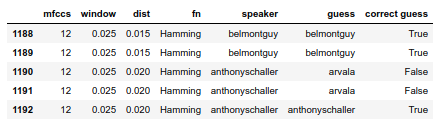
\includegraphics[height=97pt]{Figure_7.png}
        % \caption{}
    \end{figure}

\end{frame}



\section{Resultados}

\begin{frame}
    \frametitle{Análise dos parâmetros: número de MFCCs}

    \begin{figure}[]
        \centering
        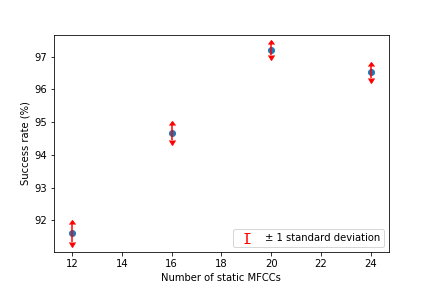
\includegraphics[height=192pt]{Figure_1.png}
        % \caption{}
    \end{figure}

\end{frame}

\begin{frame}
    \frametitle{Análise dos parâmetros: intervalo de amostragem}

    \begin{figure}[]
        \centering
        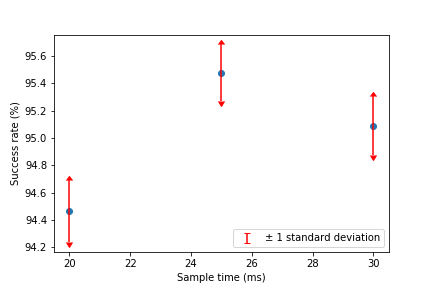
\includegraphics[height=192pt]{Figure_2.png}
        % \caption{}
    \end{figure}

\end{frame}

\begin{frame}
    \frametitle{Análise dos parâmetros: distância entre janelas}

    \begin{figure}[]
        \centering
        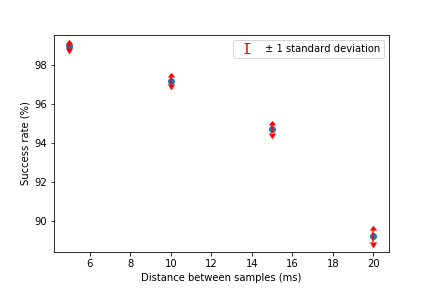
\includegraphics[height=192pt]{Figure_3.png}
        % \caption{}
    \end{figure}

\end{frame}
\begin{frame}
    \frametitle{Análise dos parâmetros: função de janelamento}

    \begin{figure}[]
        \centering
        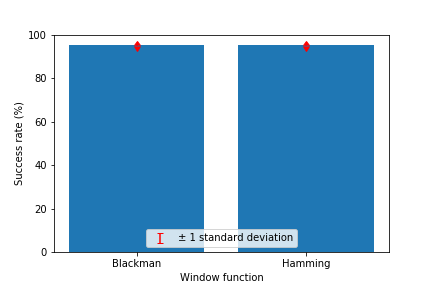
\includegraphics[height=192pt]{Figure_4.png}
        % \caption{}
    \end{figure}

\end{frame}
\begin{frame}
    \frametitle{Análise dos parâmetros: correlação linear}

    \begin{figure}[]
        \centering
        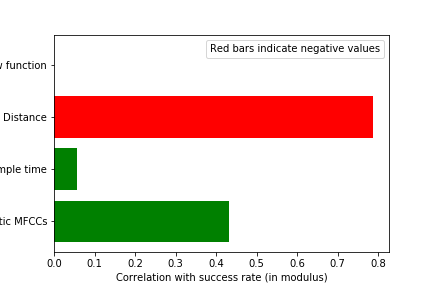
\includegraphics[height=192pt]{Figure_5.png}
        % \caption{}
    \end{figure}

\end{frame}
\begin{frame}
    \frametitle{Análise dos parâmetros: piores e melhores combinações}

    \begin{figure}[]
        \centering
        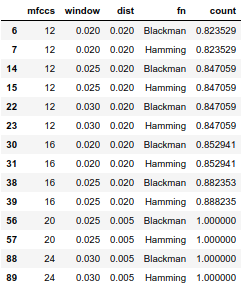
\includegraphics[height=192pt]{Figure_6.png}
        % \caption{}
    \end{figure}

\end{frame}



% \section{Referências bibliográficas}

% \begin{frame} % SLIDE 53
%     \frametitle{Referências bibliográficas}
%     \footnotesize{
%     \begin{thebibliography}{99} % Beamer does not support BibTeX so references must be inserted manually as below
%     % \bibitem[Smith, 2012]{p1} John Smith (2012)
%         \bibitem[Silberschatz, 2010]{p1}
%         Silberschatz, A., Korth, H. F., \& Sudarshan, S. (2010). Database system concepts (Vol. 4). New York: McGraw-Hill.

%         \bibitem[Rawat, 2017]{p2}
%         Rawat, U. (2017). Implementation of Locking in DBMS. Acessado a \date{25/11/2018} em https://www.geeksforgeeks.org/implementation-of-locking-in-dbms/.

%         \bibitem[Porfirio, 2013]{p3}
%         Porfirio, Alice \& Pellegrini, Alessandro \& Di Sanzo, Pierangelo \& Quaglia, Francesco. (2013). Transparent Support for Partial Rollback in Software Transactional Memories. 8097. 583-594. 10.1007/978-3-642-40047-6\_59. 

%         \bibitem[Poddar, 2013]{p4}
%         Poddar, Saumendra. (2003). SQL Server Transactions and Error Handling. Acessado a \date{25/11/2018} em https://www.codeproject.com/Articles/4451/SQL-Server-Transactions-and-Error-Handling.
%     \end{thebibliography}
%     }
% \end{frame}


% \begin{frame} % SLIDE 53
%     \frametitle{Referências bibliográficas}
%     \footnotesize{
%     \begin{thebibliography}{99} % Beamer does not support BibTeX so references must be inserted manually as below

%     \bibitem[Singhal, 2018]{p5}
%         Singhal, Akshay. (2018). Cascading Schedule | Cascading Rollback | Cascadeless Schedule. Acessado a \date{25/11/2018} em https://www.gatevidyalay.com/cascading-schedule-cascading-rollback-cascadeless-schedule/.

%         \bibitem[Pandey, 2018]{p6}
%         Pandey, Anand. (2018). Transactions and Concurrency Control. Acessado a \date{25/11/2018} em https://gradeup.co/transactions-and-concurrency-control-i-4c5d9b27-c5a7-11e5-bcc4-bc86a005f7ba.

% 	    \bibitem[Difference between, 2018]{p7}
%         Difference between. (2018). Difference between Deadlock and Starvation. Acessado a \date{25/11/2018} em http://www.differencebetween.info/difference-between-deadlock-and-starvation.

%     \end{thebibliography}
%     }
% \end{frame}

%------------------------------------------------

\end{document} 